\documentclass[a4j,titlepage]{jarticle}
\usepackage{epic,eepic}
\usepackage[dvipdfmx]{graphicx}
\usepackage{array}
\usepackage{amsmath}
\usepackage{tabularx}
\usepackage{float}
\usepackage{latexsym}
\usepackage{theorem}
\usepackage{url}
\usepackage{cases}
\usepackage{comment}
\usepackage{multirow}
\usepackage{color} %色
\usepackage[dvipdfmx]{hyperref} %urlの色
\usepackage{fancyhdr} %ヘッダーフッター
\usepackage{here} %図表の場所
\usepackage{listings,jlisting} %ソースコード

%url等の色を決める
\hypersetup{
    colorlinks=true,
    citecolor=black,
    linkcolor=black,
    urlcolor=blue,
}

%色の定義
%\definecolor{whatcolor}{rgb}{ rgb値, rgb値, rgb値}

%grayを定義
\definecolor{gray}{gray}{0.9}

\oddsidemargin20mm
\columnsep\textwidth
\advance\columnsep-2\columnwidth
\columnsep.5\columnsep
\advance\oddsidemargin-1in
\evensidemargin\oddsidemargin

%図表の表示
\renewcommand{\figurename}{Fig.}
\renewcommand{\tablename}{Table }
\renewcommand{\lstlistingname}{Src.}

%subsubsubsectionとsubsubsubsubsectionを定義
\setcounter{secnumdepth}{5}
\makeatletter
\newcommand{\subsubsubsection}{\@startsection{paragraph}{4}{\z@}%
{1.5\baselineskip \@plus.5\dp0 \@minus.2\dp0}%
{.5\baselineskip \@plus2.3\dp0}%
{\reset@font\normalsize\bfseries}
}
\newcommand{\subsubsubsubsection}{\@startsection{subparagraph}{5}{\z@}%
{1.5\baselineskip \@plus.5\dp0 \@minus.2\dp0}%
{.5\baselineskip \@plus2.3\dp0}%
{\reset@font\normalsize\itshape}
}
\makeatother
\setcounter{tocdepth}{5}

%ソースコードの表示に関する設定
\lstset{
  basicstyle={\ttfamily},
  identifierstyle={\small},
  commentstyle={\smallitshape},
  keywordstyle={\small\bfseries},
  ndkeywordstyle={\small},
  stringstyle={\small\ttfamily},
  frame={tb},
  breaklines=true,
  columns=[l]{fullflexible},
  numbers=left,
  xrightmargin=0zw,
  xleftmargin=3zw,
  numberstyle={\scriptsize},
  stepnumber=1,
  numbersep=1zw,
  lineskip=-0.5ex
}

\pagestyle{empty}
\newcolumntype{C}[1]{>{\centering}p{#1\linewidth}|}

\title{Bitbank自動取引}
%\etitle{英語題名}

\author{
  関藤大凱\ \
}

%\eauthor{Taiga Sekitou}
%\jaffiliation{$^{*1}$ & 岡山大学機械システム系学科システム工学コース}
%\eaffiliation{$^{*1}$ Department of Mechanical and System Engineering, Okayama Univesity}

\date{\today}

%\abstract{abstract}
%\keywords{keyword}

\pagestyle{fancy}
\lhead{} %ヘッダ左
\chead{} %ヘッダ中央
\rhead{Bitbank} %ヘッダ右.コンパイルした日付を表示
\lfoot{} %フッタ左
\cfoot{\thepage} %フッタ中央.ページ番号を表示
\rfoot{} %フッタ右
 \renewcommand{\headrulewidth}{0.5pt} %ヘッダの罫線
 \renewcommand{\footrulewidth}{0.5pt} %フッタの罫線

\begin{document}
\maketitle
\thispagestyle{empty}

%目次
\tableofcontents
\clearpage

\section{準備}
\subsection{APIの発行}
itbankのアカウント画面から「API」をクリックし,APIを発行

\subsection{python\_bitbankccのインストール}
コマンドプロンプトで以下をインストールする
\begin{center}
  \colorbox{gray}{pip install git+https://github.com/bitbankinc/python-bitbankcc.git}
\end{center}

\subsection{APIについて}
BitbankのAPIは大きく3つに分類される.
\begin{itemize}
  \item public API\\
    公開しているテイカー情報,板情報等
  \item rest API(private API)\\
    自身の注文履歴,資産残高の確認や,新規注文をする
  \item public stream API\\
    データをリアルタイムで受信・送信する
\end{itemize}
\section{パブリックAPI}

\begin{table}[htbp]
  \caption{パブリックAPI}
  \label{tab:API}
  \begin{tabular}{lll}
  関数                & 説明                                                                        & 引数                                                                       \\ \hline
  get\_ticker       & 市場価格を取得                                                                   & pair                                                                     \\
  get\_depth        & 板情報を取得                                                                    & pair                                                                     \\
  get\_transactions & \begin{tabular}[c]{@{}l@{}}最新の全約定履歴を取得\\ または、\\ 指定日の全約定履歴を取得\end{tabular} & \begin{tabular}[c]{@{}l@{}}pair\\ または\\ pair, yyyymmdd=None\end{tabular} \\
  get\_candlestick  & 指定日のロウソク足データを取得                                                           & pair, candle\_type, yyyymmdd                                            
  \end{tabular}
  \end{table}


\subsection{テイカー情報の取得}
\lstinputlisting{bitbank1.py}
sell: 現在の売り注文の最安値\\
buy: 現在の買い注文の最安値\\
high: 過去24時間の最高値取引価格\\
low: 過去24時間の最安値取引価格\\
last: 最新取引価格\\
vol: 過去24時間の出来高\\

\subsection{板情報の取得}
get\_transactionsを用いることで,約定履歴が取得可能になる.
\lstinputlisting{bitbank2.py}
get\_depthを使用することで板情報が取得可能.
ここで,valueにはdict型で「asks:list型」「bids:list型」が格納されているので,joinとmapを用いて文字列に変換している.
\newpage

\subsection{全約定履歴を取得}
\lstinputlisting{bitbank3.py}
「transcation\_id」と「execued\_at」はint型なのでstr型に変換している.また,「execued\_at」はUnixTimeのミリ表示なので,日付に変更する.そこで,datetimeをインポートし,datetime.datetime.fromtimestampを用いている.日時を指定するとその日の全約定履歴も取得可能.
\begin{lstlisting}[caption=bitbank3.5,label=bitbank3.5]
  指定した日時の全約定履歴の取得
  value = get_transactions( 'ペア' )
  を変更する
  value = get_transactions( 'ペア', 'YYYYMMDD 型の日付' )
  YYYYMMDD 型の日付例⇒20180504等
\end{lstlisting}
\newpage

\subsection{ロウソク足データの取得}
get\_candlestickを用いることで,ローソク足データが取得可能となる.
\lstinputlisting{bitbank4.py}
\section{プライベートAPI}
\begin{verbatim}
  #AIPキー
  API_KEY = '5f2d8797-5d8f-4ccb-ac3a-d2bd05d4e5ea'
  #シークレット
  API_SECRET = '216c999292e8ee068359f440cb58d5e8c895450356203cd2946f1882491a7394'
\end{verbatim}

\begin{table}[htbp]
  \caption{プライベートAPI}
  \label{tab:API}
  \begin{tabular}{lll}
  関数                     & 説明              & 引数                                     \\ \hline
  get\_asset             & 資産の一覧を取得        &                                        \\
  get\_orders            & オーダー情報を取得       & pair, order\_id                        \\
  get\_active\_orders    & アクティブなオーダー情報を取得 & pair, options=None                     \\
  order                  & オーダーを入れる        & pair, price, amount, side, order\_type \\
  cancel\_order          & オーダーをキャンセルする    & pair, order\_id                        \\
  cancel\_orders         & 複数のオーダーをキャンセルする & pair, order\_ids                       \\
  get\_orders\_info      & 複数のオーダー情報を取得    & pair, order\_ids                       \\
  get\_trade\_history    & 約定履歴を取得         & pair, order\_count                     \\
  get\_withdraw\_account & 出金アカウントを取得      & asset                                  \\
  request\_withdraw      & 出金をリクエスト        & asset, uuid, amount, token            
  \end{tabular}
  \end{table}

\newpage

\subsection{アセット情報の取得}
get.assetを用いることでアセット情報が取得可能になる.
\lstinputlisting{bitbank5.py}
valueの値を変更することで取得する情報を変更できる.
\newpage

\subsection{注文IDを指定して注文情報を取得}
get\_orderを用いることで,指定したIDの注文情報が取得可能となる. 
\lstinputlisting{bitbank6.py}
prv.get\_orders\_infoを用いることで,複数の注文IDを指定することが可能となる.
\begin{verbatim}
  単数:prv.get_order( 'ペア', '注文ID' )
  複数:prv.get_orders_info(  'ペア', ['注文ID', '注文ID', .....] )
\end{verbatim}
「注文状態」には,「UNFILLED(注文中)」「PARTIALLY\_FILLED(注文中(一部約定))」「FULLY\_FILLED(約定済み)」「CANCELED\_UNFILLED(取消済)」「CANCELED\_PARTIALLY\_FILLED(取消済(一部約定))」の5種類存在する.
\newpage

\subsection{アクティブな注文情報を取得}
get\_active\_ordersを用いることで,アクティブな注文情報が取得可能となる.
\lstinputlisting{bitbank7.py}
\newpage

\subsection{新規注文を行う}
\textcolor{red}{本当に注文が通るので,自己責任で行う}\\
orderにより,新規注文が可能となる.一方で,cancel\_orderにより,注文をキャンセル可能となる(複数キャンセルも可能).
\lstinputlisting{bitbank8.py}
\begin{verbatim}
  単数:cancel_order( 'ペア', '注文ID' )
  複数:cancel_order( 'ペア', ['注文ID', '注文ID', .....] )
\end{verbatim}
ただし,以下の様に「取引」を選択したAPIキーを発行・使用する必要があることに注意.
\begin{figure}[H]
  \centering
  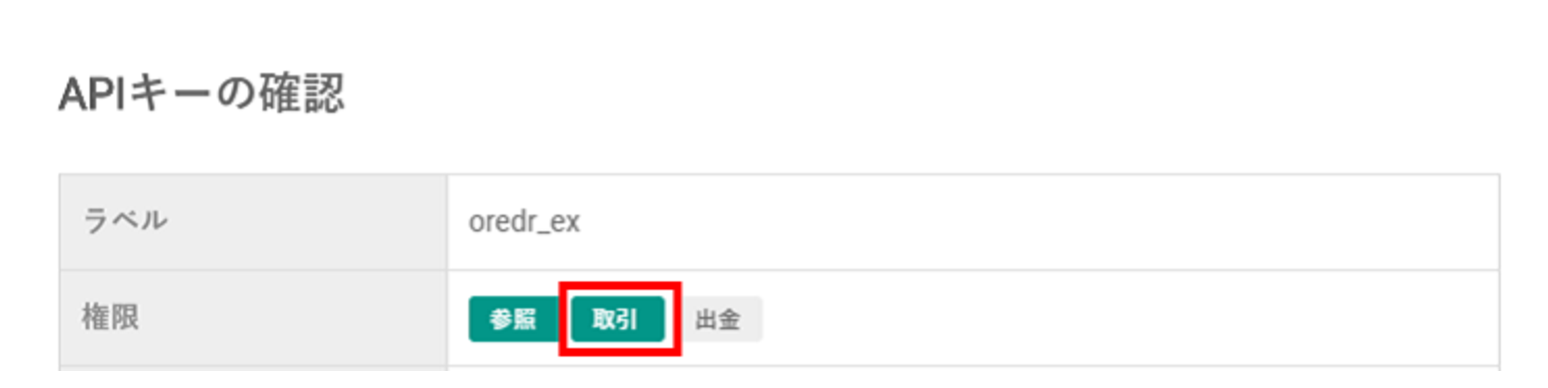
\includegraphics[width=8.0cm]{APIキーの確認.eps}
  \caption{APIキーの確認}
  \label{APIキーの確認}
\end{figure}
\newpage

\subsection{約定履歴を取得する}
\textcolor{red}{故障中?}\\
trade\_historyを使用することで約定履歴を取得できる.
\lstinputlisting{bitbank9.py}


\end{document}

